\section{Comparison: Spectrogram and Cepstrogram}
The comparison of spectrogram and cepstrogram has been performed for the combination of female speech versus music and for female speech versus male speech. The code is given by:
\begin{lstlisting}
window_length = 0.03; %in ms
num_cepstral  = 13;

[mfccs_f,spectgram_f,f_f,t_f]       = GetSpeechFeatures(y_female,...
                                fs_female,window_length,num_cepstral);
[mfccs_mu,spectgram_mu,f_mu,t_mu]   = GetSpeechFeatures(y_music,...
                                fs_music,window_length,num_cepstral);
[mfccs_ma,spectgram_ma,f_ma,t_ma]   = GetSpeechFeatures(y_male,...
                                fs_male,window_length,num_cepstral);


% mean the signal
mfccs_f = mfccs_f-repmat(mean(mfccs_f,2),1,size(mfccs_f,2));
mfccs_mu = mfccs_mu-repmat(mean(mfccs_mu,2),1,size(mfccs_mu,2));
mfccs_ma = mfccs_ma-repmat(mean(mfccs_ma,2),1,size(mfccs_ma,2));
% normalize variance to 1
norm_f   = (std(mfccs_f.')).';
mfccs_fn = mfccs_f.*repmat((1./norm_f),1,size(mfccs_f,2));
norm_m   = (std(mfccs_mu.')).';
mfccs_mn = mfccs_mu.*repmat((1./norm_m),1,size(mfccs_mu,2));
norm_ma   = (std(mfccs_ma.')).';
mfccs_man = mfccs_ma.*repmat((1./norm_ma),1,size(mfccs_ma,2));

figure(7)
subplot(2,1,1); imagesc(t_f,f_f,log10(spectgram_f)); colormap jet
xlabel('Time in seconds'); ylabel('Frequency in Hz'); title('Female voice - Spectrogram')
subplot(2,1,2); imagesc(t_mu,f_mu,log10(spectgram_mu)); colormap jet;
xlabel('Time in seconds'); ylabel('Frequency in Hz'); title('Music - Spectrogram')

figure(8)
subplot(2,1,1); imagesc(t_f,1:num_cepstral,mfccs_fn); colormap jet
xlabel('Time in seconds'); ylabel('MFCCS'); title('Female voice - Cepstrogram')
subplot(2,1,2); imagesc(t_mu,1:num_cepstral,mfccs_mn); colormap jet
xlabel('Time in seconds'); ylabel('MFCCS'); title('Music - Cepstrogram')

figure(9)
subplot(2,1,1); imagesc(t_f,f_f,log10(spectgram_f)); colormap jet
xlabel('Time in seconds'); ylabel('Frequency in Hz'); title('Female voice - Spectrogram')
subplot(2,1,2); imagesc(t_ma,f_ma,log10(spectgram_ma)); colormap jet;
xlabel('Time in seconds'); ylabel('Frequency in Hz'); title('Male voice - Spectrogram')

figure(10)
subplot(2,1,1); imagesc(t_f,1:num_cepstral,mfccs_fn); colormap jet
xlabel('Time in seconds'); ylabel('MFCCS'); title('Female voice - Cepstrogram')
subplot(2,1,2); imagesc(t_ma,1:num_cepstral,mfccs_man); colormap jet
xlabel('Time in seconds'); ylabel('MFCCS'); title('Male voice - Cepstrogram')
\end{lstlisting}

The results for the music and female speech comparison are shown in figure \ref{fig:7} and \ref{fig:8}. For a human, the spectrogram representation is easier to interpret since the all-time occurring harmonics within the music signal are very characteristic. Also, the distinction between voiced and unvoiced sounds in the speech signal are obvious. As a human, you also have kind of a physical notion for these real physical quantities that relate to certain frequencies. On the other hand, the cepstrogram is low dimensional in the sense that the amount of data has been reduced significantly, which makes it easier to handle the data within a computer. But for a human, the understanding of the pattern are much harder here. The normalised cepstrogram seems to be random on a first glance. It is hard to distinguish between voiced and unvoiced sound by looking.\\

The other comparison is shown in figure \ref{fig:9} and \ref{fig:10}. The spectrograms are similar for a human since they have kind of the same behaviour. Voiced and unvoiced parts are visible, but they are a bit blurred within the male signal. The first and third unvoiced parts are visible within the male signal, whereas these characteristic is not visible for the second unvoiced part. Also, the harmonics are more or less blurred. Hence, there are differences between the signals, but the similarities are visiblie for a human (this goes along with the fact that we know that it represents the same phrase beforehand). Due to the high amount of data and also the difference in output power and pitch between those signals, it could be hard for a computer to make this statement. The cepstrogram comparison seems random at first, but having a deeper look into it, it becomes clear that the cepstrograms share some properties, which can be handled easily by the computer. The pitch has been removed such that the harmonics don't differ anymore and also the general behaviour when comparing the coefficients are similar. For instance the third coefficient has high (red) values around $1.4$ seconds and low (blue) values around $0.4$ seconds for both male and female signal. In general it seems like the computer has an advantage here compared to a human to interpret these pictures.

\begin{figure}[h]
		\centering
		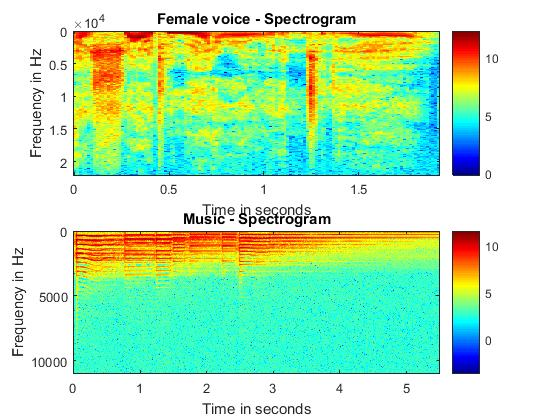
\includegraphics[width=0.77\linewidth]{./images/7.jpg}
		\caption{Spectrogram comparison: female speech vs. music signal}
		\label{fig:7}	
\end{figure}
\begin{figure}[h]
		\centering
		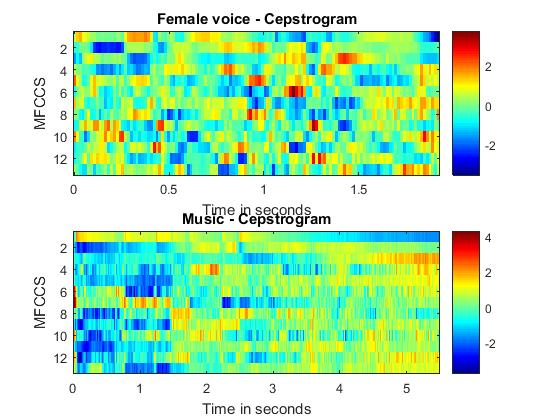
\includegraphics[width=0.75\linewidth, keepaspectratio]{./images/8.jpg}
		\caption{Cepstrogram comparison: female speech vs. music signal}
		\label{fig:8}	
\end{figure}
\pagebreak
\begin{figure}[h]
		\centering
		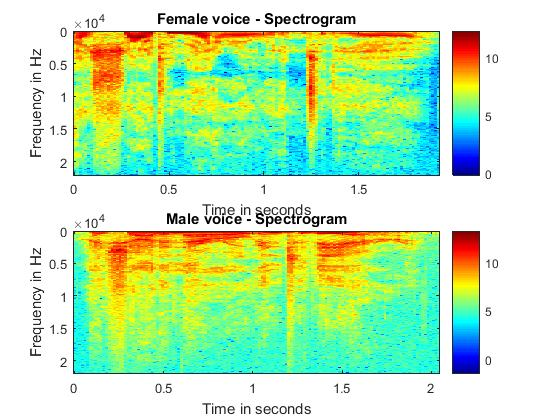
\includegraphics[width=0.75\linewidth, keepaspectratio]{./images/9.jpg}
		\caption{Spectrogram comparison: female speech vs. male speech}
		\label{fig:9}	
\end{figure}
\pagebreak
\begin{figure}[h]
		\centering
		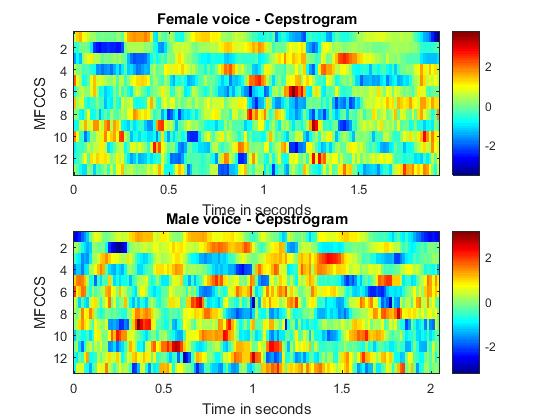
\includegraphics[width=0.75\linewidth, keepaspectratio]{./images/10.jpg}
		\caption{Cepstrogram comparison: female speech vs. male speech}
		\label{fig:10}	
\end{figure}
